
This chapter presents an overview of the actuation system model created by \citeonline{Constantino} and improved by \citeonline{Ballesteros} used in this development. Further details can be found in one of the mentioned references. 

The architecture of the hydraulic actuator modeled is shown in Figure \ref{fig:3_HydArch}. The model considers check valves, an electro-hydraulic servo valve, anti-cavitation valves and the actuator piston.

\begin{figure}[H]
	\centering
	\centerline{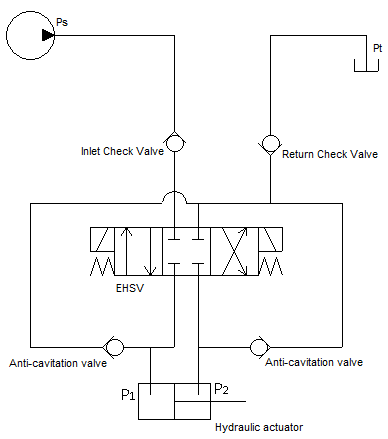
\includegraphics[width=0.5\textwidth]{Figuras/3.ActuationSystemModel/3-act_hyd_schematic.png}}
	\caption{Actuator hydraulic schematic. Source: \citeonline{Ballesteros}}
	\label{fig:3_HydArch}
\end{figure}

The actuator servo valve considered in the model is a two-stage four-way electro-hydraulic servo valve, represented in Figure \ref{fig:3_EHSV}.

\begin{figure}[H]
	\centering
	\centerline{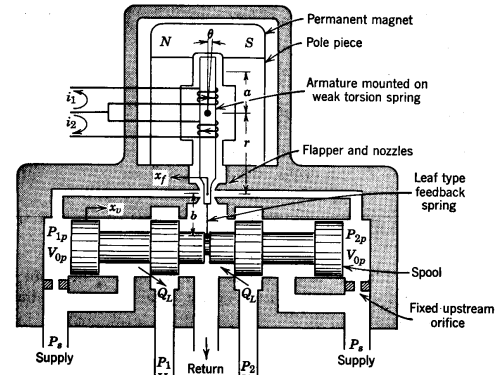
\includegraphics[width=0.8\textwidth]{Figuras/3.ActuationSystemModel/3-EHSV_moog.png}}
	\caption{Two-stage EHSV schematic. Source: \citeonline{Thayer}}
	\label{fig:3_EHSV}
\end{figure}

The following equations derived by \citeonline{Ballesteros} represent a simplified version of the non-linear system.

\begin{gather}
\dddot{x_v} = \frac{1}{A_s K_r} (K_l K_2 w_{n_e}^2 i - 2 \xi_e w_{n_e} A_s K_r \ddot{x_v} - A_s K_r w_{n_e}^2 \dot{x_v} - K_2 K_w w_{n_e}^2 x_v) \label{eq:nonlinear_ehsv2} \\
\dot{P_1} = \frac{\beta_c}{V_{01} + A_p x_p} (K_{CD} (\sqrt{P_S - P_1}(x_v x_w + A_{leak}) - \sqrt{P_1-P_T} A_{leak} - A_{ext} \sqrt{P_1} - A_{int} \sqrt{P_1-P_2}) - A_p\dot{x_p}) \label{eq:P1nonlinear2} \\
\dot{P_2} = \frac{\beta_c}{V_{02} - A_p x_p} (A_p\dot{x_p} + K_{CD}(\sqrt{P_S-P_2} A_{leak} - A_{ext} \sqrt{P_2} + A_{int} \sqrt{P_1-P_2} - \sqrt{P_2 - P_T}(x_v x_w + A_{leak}))) \label{eq:P2nonlinear2} \\
\ddot{x_p} = \frac{1}{m_p} (A_p (P_1 - P_2) - B_p \dot{x_p}) \label{eq:piston_nonlinear2}
\end{gather}
%
%Where: 
%
%\begin{description}
%	\item $x_v$: EHSV 1st stage spool position
%	\item $w_{n_e}$: EHSV 1st stage natural frequency
%	\item $\xi_{e}$: EHSV 1st stage damping ratio
%	\item $A_s$: EHSV spool end area
%	\item $K_r$: EHSV flapper-armature gain
%	\item $K_l$: EHSV 1st stage torque motor gain
%	\item $x_v$: EHSV spool displacement
%	\item $i$: EHSV current
%	\item $K_2$: Hydraulic amplifier flow gain
%	\item $K_w$: Feedback wire stiffness
%	\item $P_1$: Pressure in piston chamber 1
%	\item $P_2$: Pressure in piston chamber 2
%	\item $x_p$: Piston position
%	\item $A_p$: Piston area
%	\item $V_{01}$: Chamber 1 initial volume
%	\item $V_{02}$: Chamber 2 initial volume
%	\item $\beta_c$: Constant bulk modulus
%	\item $K_{CD}$: Constant based on the discharge coefficient and fluid density
%	\item $P_s$: Supply pressure
%	\item $P_t$: Return pressure
%	\item $A_{int}$: internal leakage equivalent area
%	\item $A_{ext}$: external leakage equivalent area
%	\item $x_{w}$: EHSV second-stage orifice area width 
%	\item $A_{leak}$: EHSV second-stage leakage
%	\item $m_p$: piston mass
%	\item $B_p$: viscous damping coefficient
%\end{description}

Defining $\Delta P = P_1 - P_2$, the equations above describe the following non-linear state space with state vector $X$ with input $U$ and output $Y$:

\begin{eqnarray}
&& \dot{X}= A X + B U \\
&& Y = C X + D U
\end{eqnarray}

\begin{center}
	$X = \begin{bmatrix}
	x_v \\
	\dot{x_v} \\
	\ddot{x_v}\\
	\Delta P\\
	x_p\\
	\dot{x_p}
	\end{bmatrix}
	$
\end{center}

\begin{center}
	$U = i$\\
\end{center}

\begin{center}
	$Y =\begin{bmatrix}
	x_v \\
	\Delta P\\
	x_p\\
	\end{bmatrix}$
\end{center}

Where the matrices A, B, C and D are obtained from the terms of the system equations.

\section{Simulink Model}

Figure \ref{fig:3_SimulinkModel} shows the actuation system interfaces and the support blocks necessary to simulate the system.

\begin{figure}[H]
	\centering
	\centerline{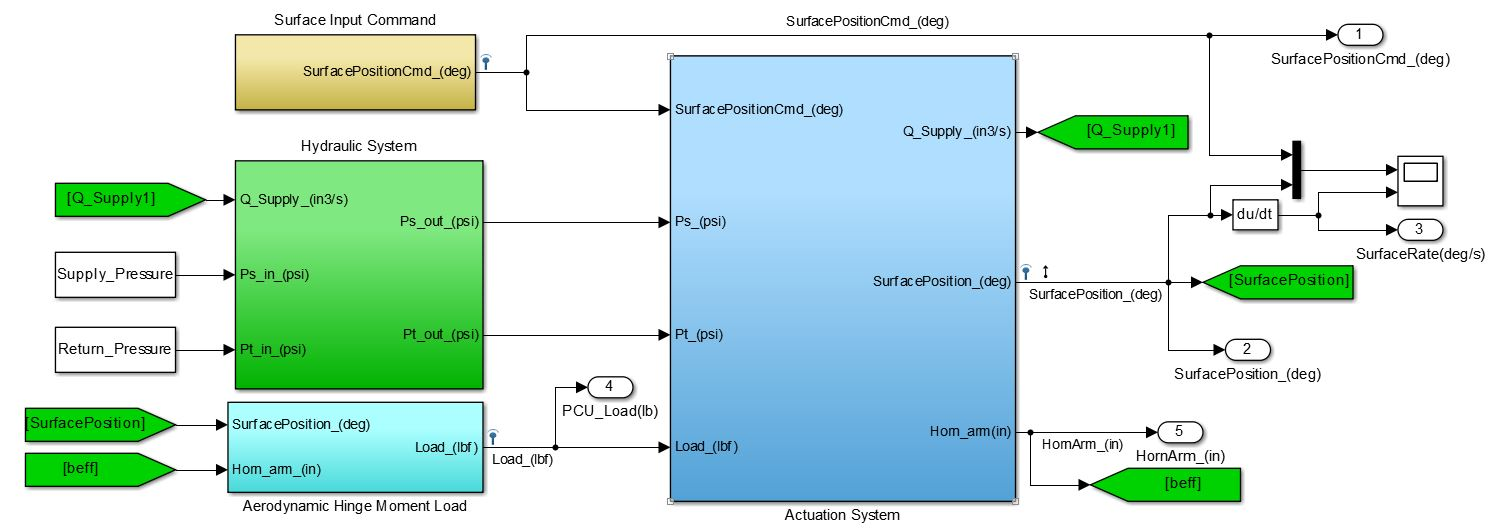
\includegraphics[width=1.1\textwidth]{Figuras/3.ActuationSystemModel/3-Model.jpg}}
	\caption{Actuation System and Interfaces Simulink Model}
	\label{fig:3_SimulinkModel}
\end{figure}

The actuation system receives the reference surface position command in degrees. This input can be configured as a null command, a repeating sequence, a sine wave, a step command, a square pulse or a square sine.

Hydraulic power is also provided through the supply and return pressure inputs. The hydraulic system model is configured to provide a nominal supply pressure of 3000psi and 150psi at the return line. Since the fluid inertia has been considered, these values may fluctuate depending on the fluid flow consumed by the actuator.

Another input of the actuation system is the aerodynamic load at the actuator piston. This parameter may be configured as a sine wave, used for the dynamic stiffness test, a linear load as a function of the surface position and a constant value.

The actuation system outputs are the consumed hydraulic fluid flow, the control surface position and the horn arm which is also considered to calculated the linear aerodynamic load.

The actuation system is divided in three parts as shown in Figure \ref{fig:3_ActuationSystem}: electronic system, actuator and surface kinematics.

\begin{figure}[H]
	\centering
	\centerline{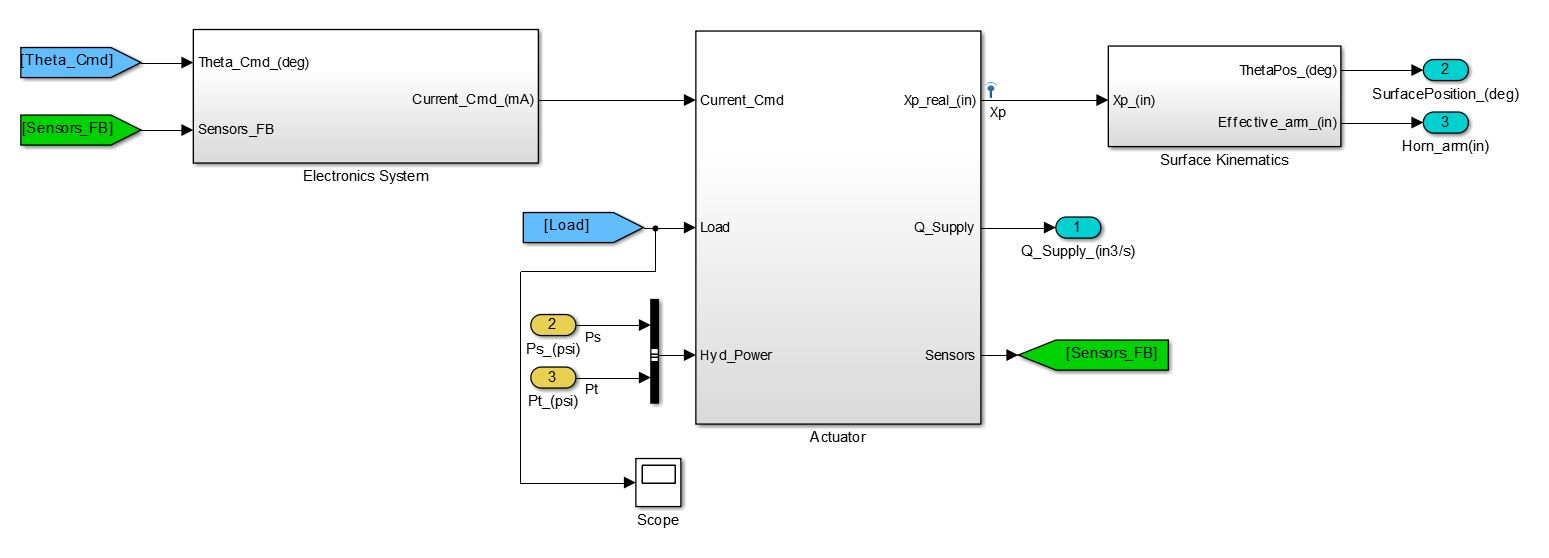
\includegraphics[width=1.1\textwidth]{Figuras/3.ActuationSystemModel/3-ActuationSystem.jpg}}
	\caption{Actuation System Simulink Model}
	\label{fig:3_ActuationSystem}
\end{figure}

The electronics system receives the surface command input and the feedback sensors from the actuator. These sensors are LVDTs that measure the piston position, the differential pressure in the cylinder and the EHSV (Electro-Hydraulic Servo Valve) displacement.

The actuator receives a current command from the electronic system, the hydraulic supply and return pressures and the aerodynamic load at the piston. These inputs are used to calculate piston position and the fluid flow consumed by the actuator. Finally, the control surface position and horn arm are calculated from the piston position. 

The following sections detail the characteristics modeled in each of these three parts.

\subsection{Electronic System}

The electronic system model is shown in Figure \ref{fig:3_1_ElectronicSystem}.

\begin{figure}[H]
	\centering
	\centerline{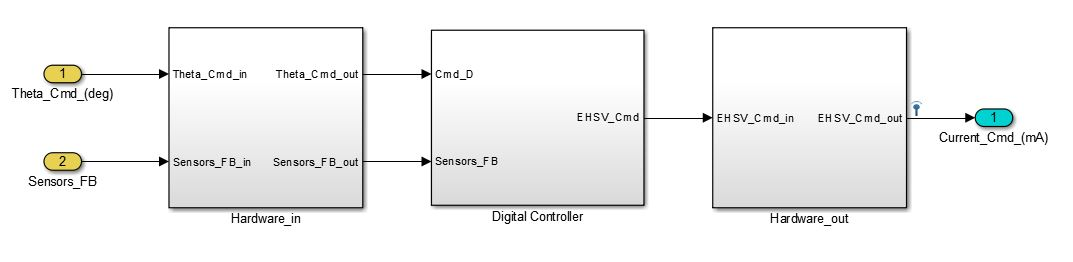
\includegraphics[width=1.1\textwidth]{Figuras/3.ActuationSystemModel/3-1-ElectronicSystem.jpg}}
	\caption{Electronic System Simulink Model}
	\label{fig:3_1_ElectronicSystem}
\end{figure}

The first part of the electronic system is an analog-to-digital converter which is necessary because a digital controller has been modeled and the input is analog. At this step, the signal sampling rate is set and a conversion noise is added.

The position command received by the controller is converted from degrees to millimeters prior to the subtraction of the piston position received from the LVDT sensor. An error signal is generated from this operation and sent to a PID controller that calculates a current command to be sent to the EHSV. This output is limited due to the saturation observed in real controllers.

The digital PID controller is implemented as shown in Figure \ref{fig:3_1_PID}

\begin{figure}[H]
	\centering
	\centerline{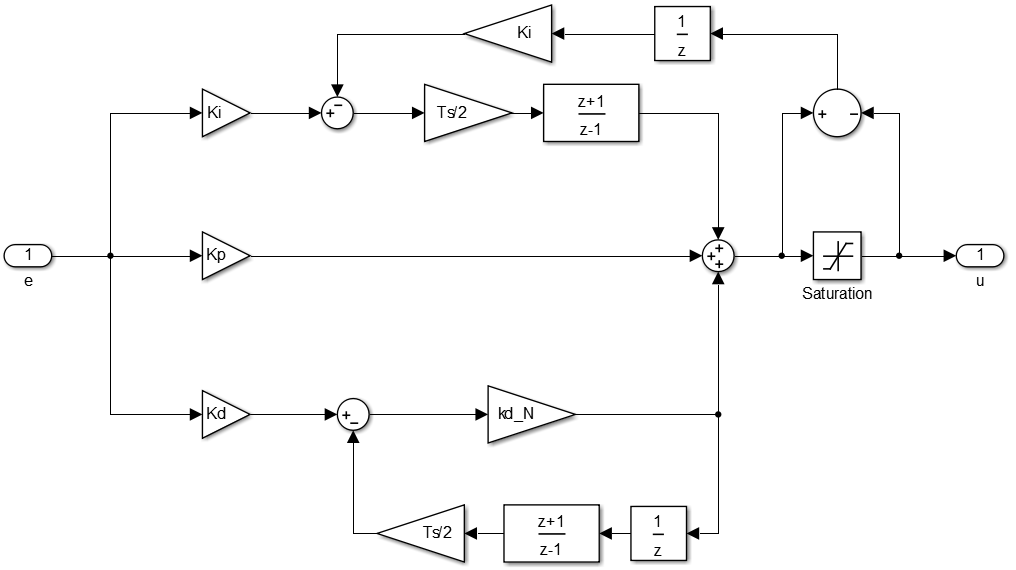
\includegraphics[width=1.1\textwidth]{Figuras/3.ActuationSystemModel/3-PID_discrete.png}}
	\caption{Digital PID Controller Model}
	\label{fig:3_1_PID}
\end{figure}

Finally, the digital current value is converted to an analog signal with power to drive the first stage of the EHSV.

\subsection{Actuator}

The actuator model is composed by valves, cylinder and sensors dynamics as shown in Figure \ref{fig:3_2_Actuator}.

\begin{figure}[H]
	\centering
	\centerline{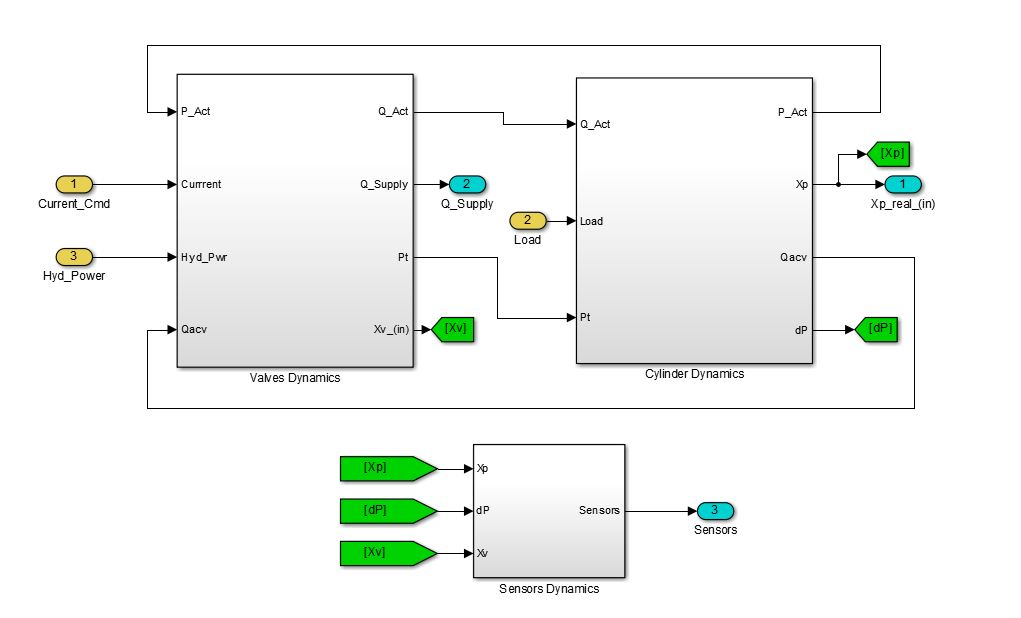
\includegraphics[width=1.1\textwidth]{Figuras/3.ActuationSystemModel/3-2-Actuator.jpg}}
	\caption{Actuator Simulink Model}
	\label{fig:3_2_Actuator}
\end{figure}

The first stage of the actuator is a set composed of two inlet check valves and an EHSV as shown in Figure \ref{fig:3_2_Valves}. The inlet check valves guarantee that no fluid will flow to the supply line and from the return line. The bulk modulus effect is considered at supply and return hydraulic lines. 

The EHSV is responsible for delivering fluid flow to the cylinder depending on the current command, hydraulic power available and the pressure at both cylinder chambers. Several non linearities are considered in the EHSV first stage, such as torque motor current saturation and flapper and spool displacement limits.

Based on the spool displacement generated at the EHSV first stage, the second stage calculates the flow between hydraulic lines and cylinder chambers as well as flow resulting from leaks. 

\begin{figure}[H]
	\centering
	\centerline{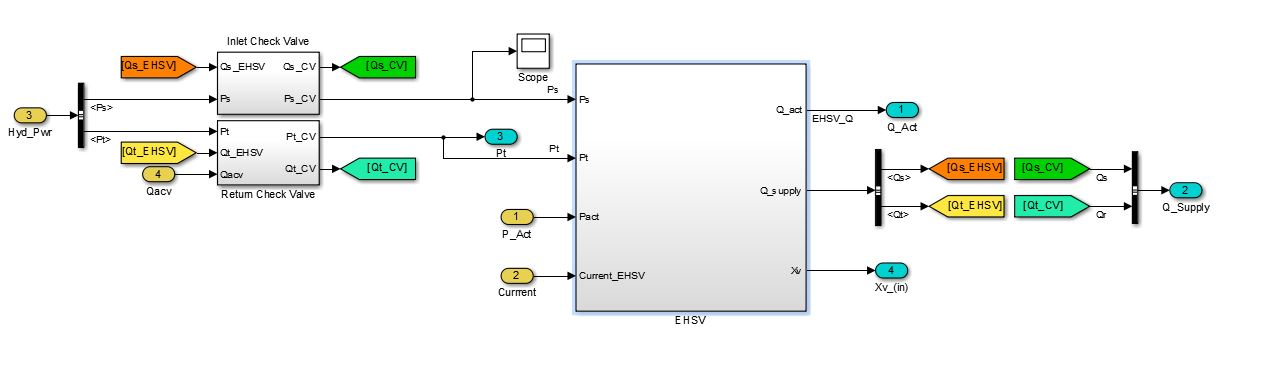
\includegraphics[width=1.1\textwidth]{Figuras/3.ActuationSystemModel/3-2-Valves.jpg}}
	\caption{Actuator Valves Simulink Model}
	\label{fig:3_2_Valves}
\end{figure}

The second stage of the actuator is composed by fluid and piston dynamics (Figure \ref{fig:3_2_Cylinder}). The fluid dynamics stage uses the flow at the cylinder chambers and the piston position to calculate the pressure at each chamber, also considering the bulk modulus effect in these volumes. Anti cavitation valves are also implemented and the flow from them is considered when calculating the flow to the return line.

The position of the piston is obtained at the piston dynamics stage based on the forces acting on it, that are: hydraulic force due to the pressure difference between cylinder chambers, damping force due to fluid viscosity, friction force at the seal and the force due to the aerodynamic load at the control surface.

\begin{figure}[H]
	\centering
	\centerline{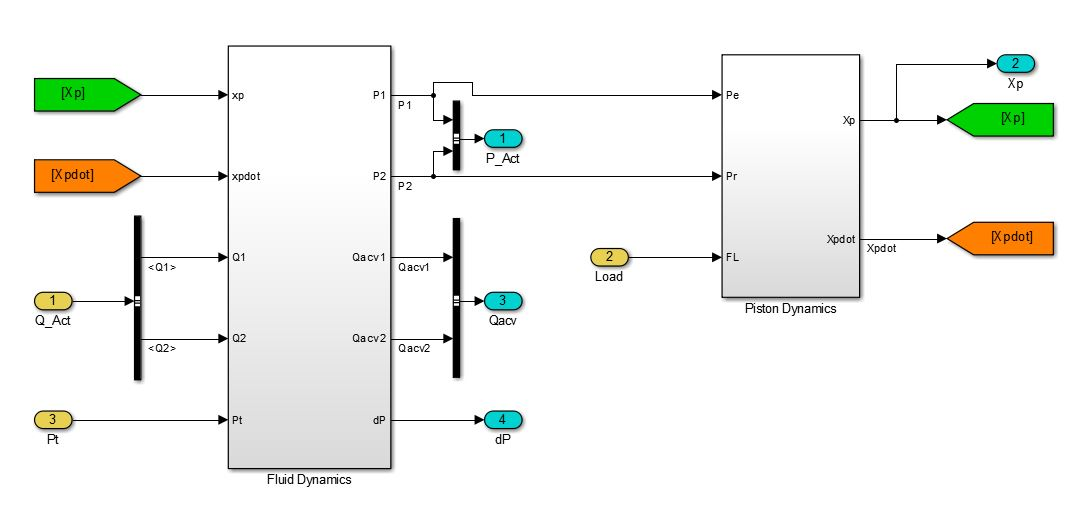
\includegraphics[width=1.1\textwidth]{Figuras/3.ActuationSystemModel/3-2-Cylinder.jpg}}
	\caption{Actuator Cylinder Simulink Model}
	\label{fig:3_2_Cylinder}
\end{figure}

The piston position, spool position and delta pressure at the cylinder are measured by LVDTs (Figure \ref{fig:3_2_Sensors}). The dynamics of these sensors are also modeled withing the actuator considering the sensor's bandwidth, range, error and hysteresis. The measured signals are fed back to the digital controller.

\begin{figure}[H]
	\centering
	\centerline{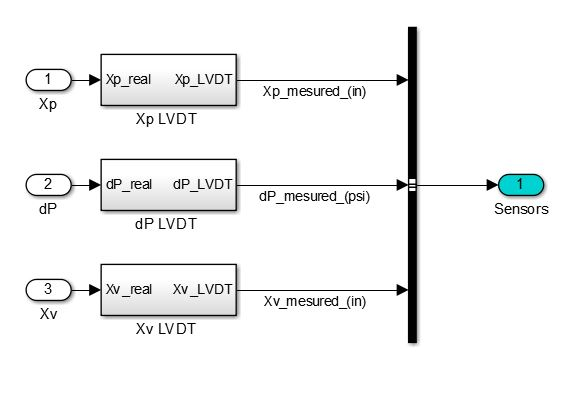
\includegraphics[width=0.6\textwidth]{Figuras/3.ActuationSystemModel/3-2-Sensors.jpg}}
	\caption{Actuator LVDT Sensors Simulink Model}
	\label{fig:3_2_Sensors}
\end{figure}

\subsection{Surface Kinematics}

The surface kinematics block only performs the conversion between linear piston movement, from the actuator, to angular control surface movement. The effective arm is also calculated to be provided to the aerodynamic load block.

Originally, the surface kinematics also considered a dynamic rotational model \cite{Constantino} but this feature was removed by \citeonline{Ballesteros} since it was not required for actuator dynamic stiffness performance evaluation.

However, the surface dynamics influence other performance characteristics such as step and frequency response. For example, when considering the control surface inertia overshoot tends to increase in the step response. Despite this, these dynamics where not consider in order to allow a fair comparison between the results achieved by \citeonline{Ballesteros} and in this development.

